\documentclass[a4paper,ngerman,12pt]{scrartcl}

\usepackage[utf8]{inputenc}
%\usepackage[ansinew]{inputenc}

\usepackage[ngerman]{babel}

\usepackage{amsmath,amsthm,amssymb,mathtools,stmaryrd,color,graphicx}
\usepackage{setspace}
\usepackage{bussproofs}
\usepackage{array}
\usepackage{comment}
\usepackage{wrapfig}

\usepackage{enumitem}

\usepackage{units}

\usepackage[protrusion=true,expansion=true]{microtype}

\usepackage{lmodern}

\usepackage{hyperref}
\usepackage{cleveref}

\newcommand{\IR}{\mathbb{R}}
\newcommand{\IC}{\mathbb{C}}
\newcommand{\IZ}{\mathbb{Z}}
\newcommand{\IN}{\mathbb{N}}
\newcommand{\IQ}{\mathbb{Q}}

\setlength\parskip{\medskipamount}
\setlength\parindent{0pt}

\theoremstyle{definition}
\newtheorem{defn}{Definition}[]
\newtheorem{axiom}[defn]{Axiom}
\newtheorem{bsp}[defn]{Beispiel}

\RequirePackage{framed}
\newtheorem{aufg}{Aufgabe}
\definecolor{shadecolor}{rgb}{.96,.96,.96}
\newenvironment{aufgabe}[1][]
		{\begin{shaded}\vspace{-0.3cm}\begin{aufg}\emph{#1} \par\medskip}
		{\end{aufg}\vspace{-0.3cm}\end{shaded}}
\newtheorem{zaufg}{Zusatzaufgabe}
	
\newenvironment{spiel}[1][]{\begin{framed}\textbf{#1:}\\}{\end{framed}}


\theoremstyle{plain}
\newtheorem{prop}[defn]{Proposition}
\newtheorem{motto}[defn]{Motto}
\newtheorem{wunder}[defn]{Wunder}
\newtheorem{ueberlegung}[defn]{Überlegung}
\newtheorem{lemma}[defn]{Lemma}
\newtheorem{kor}[defn]{Korollar}
\newtheorem{hilfsaussage}[defn]{Hilfsaussage}
\newtheorem{satz}[defn]{Satz}
\newtheorem{frage}[defn]{Frage}

\theoremstyle{remark}
\newtheorem{bem}[defn]{Bemerkung}
\newtheorem{beob}[defn]{Beobachtung}

	
\newtheorem*{antwort}{Antwort}

%\newlength{\aufgabenskip}
%\setlength{\aufgabenskip}{1.4em}
%\newcounter{aufgabennummer}
%\newenvironment{aufgabe}[1]{
%	\addtocounter{aufgabennummer}{1}
%	\textbf{Aufgabe \theaufgabennummer.} \emph{#1} \par
%}{\vspace{\aufgabenskip}}

\clubpenalty=10000
\widowpenalty=10000
\displaywidowpenalty=10000

\setlength\unitlength{1cm}

\usepackage{tikz}
\usetikzlibrary{calc}
\usepackage{tkz-euclide}
\usepackage{adjustbox}
\usepackage{algorithm2e}
\usepackage{pgfplots}

\RequirePackage{geometry}
\geometry{textwidth=17.0cm,textheight=25cm,footskip=1.5cm}


\newcommand{\kante}[2]{#1{-}#2}
\newcommand{\edge}[3]{\draw[thick] (#1) --node[rectangle,fill=gray!10]{$#3$} (#2);}

\begin{document}
	
\begin{picture}(0,0)
\put(0,-0.5){%
	
\includegraphics[scale=0.1]{logo-ifm}
}
\put(14.0,-3.5){%
	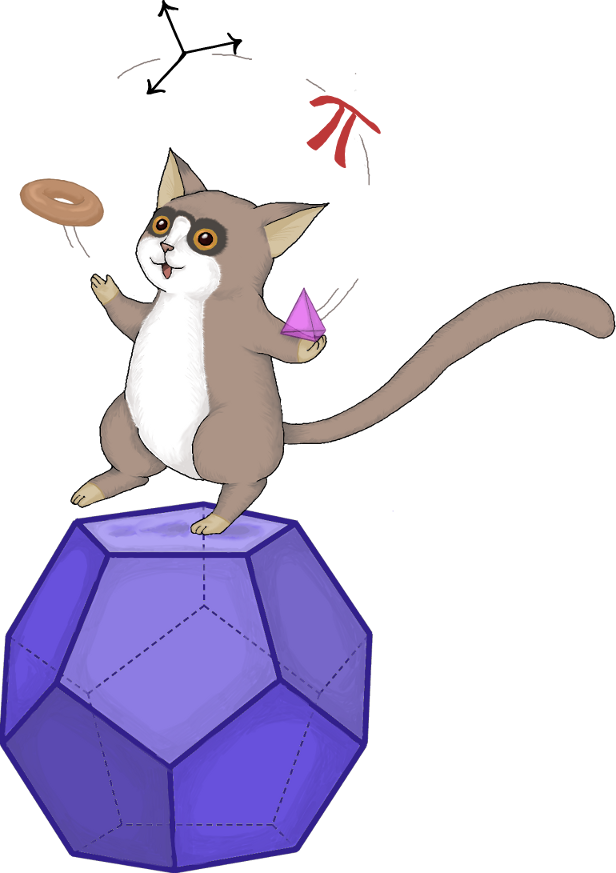
\includegraphics[scale=0.17]{cover}
}
\end{picture} 
	
\vspace{6em}

\begin{center}\Large{Mathe-Camp 2023}

\section*{Additionstheoreme für Sinus und Cosinus}\end{center}

Wir betrachten eine allgemeine Funktion $f: \IR \to \IR$. Ein \emph{Additionstheorem} für diese Funktion~$f$ ist eine Rechenvorschrift, die uns erlaubt $f(x+y)$ zu berechnen -- typischerweise nur in Termen von $f(x)$ und $f(y)$.

\begin{bsp}
	Ist $f(x) = a\cdot x$ (für irgendeine feste reelle Zahl $a \in \IR$), so gilt das folgende besonders einfache Additionstheorem:	
		\[f(x+y) = f(x)+f(y).\]
\end{bsp}
\begin{bsp}
	Eine weitere Funktion mit einem schönen Additionstheorem ist die Exponentialfunktion $f(x) = e^x$. Für diese gilt:
		\[f(x+y) = f(x)\cdot f(y).\]
\end{bsp}

Wir wollen uns heute auf die Suche nach einem solchen Additionstheorem für die Funktionen $\sin$ und $\cos$ machen.

\section{Grundlegende Eigenschaften von Sinus und Cosinus}

Wir betrachten ein rechtwinkliges Dreieck~$ABC$ mit Hypotenuse $AC$ (also rechtem Winkel bei $C$). Sei $\alpha$ der Winkel bei $A$ und $1$ die Länge der Hypotenuse. Dann definieren wir Sinus und Cosinus von $\alpha$ als die Länge der Gegen- bzw. Ankathete von $\alpha$, also:
	\[\sin(\alpha) \coloneqq \overline{BC} \quad\text{ und }\quad \cos(\alpha) \coloneqq \overline{AB}.\]
In dem folgenden Bild ist das veranschaulicht:
	\begin{center}
		\begin{tikzpicture}[scale=3]
			\draw[->,thick](-1.2,0) -- (1.2,0) node[below]{$x$};
			\draw[ultra thick](1,-.05) -- ++(0,.1) node[above right]{$1$};
			\draw[->,thick](0,-1.2) -- (0,1.2) node[right]{$y$};
			\draw[ultra thick](.05,1) -- ++(-.1,0) node[above left]{$1$};
			\draw[thick](0,0) circle (1);
			\coordinate(A) at(0,0) {};
			\node at($(A)+(-.1,-.1)$){$A$};
			\coordinate(B) at(0.866,0) {};
			\node at($(B)+(.05,-.1)$){$B$};
			\coordinate(C) at(0.866,0.5) {};
			\node at($(C)+(.1,.1)$){$C$};
			\draw[thick](A) -- (B) -- (C) --cycle;
			
			\tkzMarkAngle[size=0.5cm, mark=none](B,A,C)
			\tkzLabelAngle[pos = 0.4](B,A,C){$\alpha$} 
			
			\draw[ultra thick,blue](A) -- node[below]{$\cos(\alpha)$}(B);
			\draw[ultra thick,red](B) -- node[right=.3]{$\sin(\alpha)$}(C);
		\end{tikzpicture}
	\end{center}
In diesem Bild ist zusätzlich ein Kreis mit Radius $1$ mit dem Koordinatenursprung als Mittelpunkt eingezeichnet -- der sogenannte \emph{Einheitskreis}. Außerdem haben wir das Dreieck $ABC$ so platziert, dass $A$ im Ursprung liegt, $B$ auf der $x$-Achse und $C$ auf dem Einheitskreis.

Aus diesem Bild lässt sich leicht ableiten, wie die Funktionsgraphen von $\sin$ und $\cos$ aussehen:
\begin{center}
	\begin{tikzpicture}[scale=1.7]
		\draw[->,thick](-3.2,0) -- (3.4,0) node[below]{$\alpha$};
		\draw[thick](-3,-.1) -- ++(0,.2) node[above]{$-\tfrac{3\pi}{2}$}; 
		\draw[thick](-2,-.1) -- ++(0,.2) node[above]{$-\pi$}; 
		\draw[thick](-1,-.1) -- ++(0,.2) node[above]{$-\tfrac{\pi}{2}\,$}; 
		\draw[thick](1,-.1) -- ++(0,.2) node[above]{$\tfrac{\pi}{2}$}; 
		\draw[thick](2,-.1) -- ++(0,.2) node[above]{$\pi$}; 
		\draw[thick](3,-.1) -- ++(0,.2) node[above]{$\tfrac{3\pi}{2}$}; 
		
		\draw[->,thick](0,-1.2) -- (0,1.4);
		\draw[thick](.1,-1) -- ++(-.2,0) node[left]{$-1$}; 
		\draw[thick](.1,1) -- ++(-.2,0) node[left=.2]{$1$};
		
		\draw[dashed](-3,1) -- (3,1) (-3,-1) -- (3,-1);
		
		\draw[thick, red] (-3,1) node[above]{$\sin(\alpha)$} cos (-2,0) sin (-1,-1) cos (0,0) sin (1,1) cos (2,0) sin (3,-1);
		\draw[thick, blue] (-3,0) sin (-2,-1) node[below]{$\cos(\alpha)$} cos (-1,0) sin (0,1) cos (1,0) sin (2,-1) cos (3,0);
	\end{tikzpicture}
\end{center}

Einige wichtige Eigenschaften von Sinus und Cosinus können wir direkt an diesen Bildern sehen:
\begin{itemize}
	\item $\sin(-\alpha) = -\sin(\alpha)$
	\item $\cos(-\alpha) = \cos(\alpha)$
	\item $\sin(\alpha+\frac{\pi}{2}) = \cos(\alpha)$
	\item $\cos(\alpha + \pi) = \-\cos(\alpha)$
	\item $\sin^2(\alpha) + \cos^2(\alpha) = 1$
\end{itemize}

\begin{aufg}
	Beweise diese Eigenschaften geometrisch.
\end{aufg}

\begin{beob}
	Sei $ABC$ ein rechtwinkliges Dreieck mit Hypotenuse $AC$. Wenn die Hypotenuse eine Länge von $c$ hat und $\alpha$ der Winkel bei $A$ ist, so gilt $\overline{BC}=\sin(\alpha)\cdot c$ und $\overline{AB}=\cos(\alpha)\cdot c$.
\end{beob}

\section{Ein Geometrischer Beweis}

Mit Hilfe der folgenden Zeichnung können wir die Additionstheoreme für Sinus und Cosinus geometrisch beweisen:
\begin{center}
	\begin{tikzpicture}[scale=4]
		\draw[->,thick](-1.2,0) -- (1.2,0) node[below]{$x$};
		\draw[->,thick](0,-1.2) -- (0,1.2) node[right]{$y$};
		\draw[thick](0,0) circle (1);
		\coordinate(O) at(0,0);
		\coordinate(A) at(0.866,0.5);
		\coordinate(B) at(0.94,-0.342);
		\coordinate(1) at (1,0);
		
		\tkzMarkAngle[size=0.45cm, mark=none](1,O,A)
		\tkzLabelAngle[pos = 0.35](1,O,A){$\alpha$} 
		\tkzMarkAngle[size=0.5cm, mark=none](B,O,1)
		\tkzLabelAngle[pos = 0.35](B,O,1){$\beta$} 
		
		\draw[thick](O) -- (A);
		\draw[thick](A) -- (A |- O) coordinate(A');
		\tkzMarkRightAngle[german,size=.08](1,A',A);
		
		\draw[thick](O) -- (B);
		\draw[thick](A') -- ($(O)!(A')!(B)$) coordinate(B');
		\tkzMarkRightAngle[german,size=.08](B,B',A');
		\draw[thick](A) -- ($(O)!(A)!(B)$) coordinate(B'');
		\tkzMarkRightAngle[german,size=.08](A,B'',O);
		
		\draw[thick](A') -- ($(A)!(A')!(B'')$) coordinate(A'');
		\tkzMarkRightAngle[german,size=.08](A',A'',A);
	\end{tikzpicture}
\end{center}
Sie lauten:
	\[\cos(\alpha+\beta) = \cos(\alpha)\cos(\beta)-\sin(\alpha)\sin(\beta)\]
und
	\[\sin(\alpha+\beta) = \cos(\alpha)\sin(\beta) + \sin(\alpha)\cos(\beta).\]
	
\begin{aufg}
	Beweise die beiden Additionstheoreme. Du kannst sie entweder beide mit Hilfe der Zeichnung beweisen oder du nutzt die Zeichnung nur für eines der beiden und leitest das andere dann mit Hilfe der elementaren Eigenschaften von Sinus und Cosinus daraus her.
\end{aufg}

\begin{zaufg}
	Finde ein Additionstheorem für den Tangens. Du kannst dafür die Additionstheoreme für Sinus und Cosinus sowie die Eigenschaft $\tan(\alpha) = \frac{\sin(\alpha)}{\cos(\alpha)}$ verwenden.
	
	Alternativ kannst du auch versuchen einen direkten geometrischen Beweis zu finden. Das ist aber evtl. schwer (ich habe jedenfalls noch keine passende Zeichnung gefunden).
\end{zaufg}
	
\section{Folgerungen aus den Additionstheoremen}

\begin{aufg}
	Berechne $\cos(\alpha-\beta)$ und $\sin(\alpha-\beta)$. Entweder mit Hilfe der bereits bekannten Additionstheoreme oder mit folgender Zeichnung:
	\begin{center}
		\begin{tikzpicture}[scale=6]
			\coordinate[label=below left:$A$](A) at (0,0);
			\coordinate[label=below right:$B$](B) at (0.866,0);
			\coordinate[label=right:$C$](C) at (0.866,.5);
			\draw[thick] (A) -- (B) -- (C) --node[above]{$1$} cycle;
			
			\coordinate (E') at (.3,1);
			\draw[thick](C) -- ($(E')!(C)!(A)$) coordinate[label=above:$E$](E);
			\draw[thick](A) -- (E);
			\coordinate[label=above right:$D$](D)at($(B)!(E)!(C)$);
			\coordinate[label=above left:$F$](F)at($(A)!(E)!(0,1)$);
			\draw[thick](C)--(D)--(F)--(A);
			
			\tkzMarkAngle[size=0.25cm, mark=none](B,A,E)
			\tkzLabelAngle[pos = 0.2](B,A,E){$\alpha$} 
			\tkzMarkAngle[size=0.35cm, mark=none](C,A,E)
			\tkzLabelAngle[pos = 0.3](C,A,E){$\beta$} 
			
			\tkzMarkRightAngle[german,size=.08](C,B,A);
			\tkzMarkRightAngle[german,size=.08](A,E,C);
			\tkzMarkRightAngle[german,size=.08](F,D,B);
			\tkzMarkRightAngle[german,size=.08](A,F,D);
			\tkzMarkRightAngle[german,size=.08](B,A,F);
		\end{tikzpicture}
	\end{center}
\end{aufg}

Eine direkte Folgerung aus den Additionstheoremen sind die Formeln für die Doppelwinkelfunktionen:

\begin{lemma}
	Es gilt:
		\[\sin(2\alpha) = 2\sin(\alpha)\cos(\alpha) \quad\text{ und }\quad \cos(2\alpha) = 2\cos^2(\alpha)-1.\]
\end{lemma}

\begin{aufg}
	Beweise die Gleichheit für Cosinus. Entweder mit Hilfe des entsprechenden Additionstheorems oder mit folgender Zeichnung:
	\begin{center}
		\begin{tikzpicture}[scale=6]
			\coordinate(O) at (0,0);
			\coordinate(A) at (1.2,.5);
			\coordinate(B) at (1.2,-.5);
			\coordinate(C) at (1.2,0);
			
			\draw[thick] (O) -- node[above]{$1$} (A) -- (B) --node[below]{$1$} cycle;
			\draw[thick] (O) -- (C);
			
			\tkzMarkAngle[size=0.3cm, mark=none](C,O,A)
			\tkzLabelAngle[pos = 0.25](C,O,A){$\alpha$} 
			\tkzMarkAngle[size=0.3cm, mark=none](B,O,C)
			\tkzLabelAngle[pos = 0.25](B,O,C){$\alpha$} 
			
			\draw[thick] (A) -- ($(O)!(A)!(B)$) coordinate(A');
			\tkzMarkRightAngle[german,size=.08](A,A',O);
			
			\draw[thick] (C) -- ($(O)!(C)!(B)$) coordinate(C');
			\tkzMarkRightAngle[german,size=.08](B,C',C);
		\end{tikzpicture}
	\end{center}
\end{aufg}

\begin{zaufg}
	Beweise die Gleichheit für Sinus. Für einen geometrischen Beweis musst du dir hier selbst eine passende Zeichnung überlegen.
\end{zaufg}

\begin{zaufg}
	Zeige mit Hilfe der Additionstheoreme die Identität 
		\[\sin(\alpha)\cdot\sin(\beta) = \tfrac{1}{2}\cdot\big(\cos(\alpha-\beta)-\cos(\alpha+\beta)\big).\]
		Kannst du eine analoge Identität für $\cos$ finden?
\end{zaufg}

Mit Hilfe von Induktion sowie den Additionstheoremen und den Formeln für die Doppelwinkelfunktionen erhalten wir das folgende Lemma:

\begin{lemma}\label{lemma:MultiWinkelAlsCosinusPolynom}
	Für jede natürliche Zahl $n \in \IN$ können wir $\cos(n\cdot\alpha)$ als Polynom in $\cos(\alpha)$ schreiben (also als Summe von Vielfachen von Produkten von $\cos(\alpha)$).
\end{lemma}

\begin{aufg}
	Beweise \Cref{lemma:MultiWinkelAlsCosinusPolynom}.
	
	\textit{Tipp:} Verwende vollständige Induktion. Zeige also zunächst (Induktionsanfang), dass die Aussage für $n=1$ gilt. Zeige dann (Induktionsschritt), dass die Aussage für $n$ gilt, wenn sie für alle kleineren $n'$ bereits gilt. Im Induktionsschritt bietet es sich an zwischen $n$ gerade und $n$ ungerade zu unterscheiden.
\end{aufg}

\begin{aufg}
	Bestimme nun konkret $\cos(3\alpha)$. 
\end{aufg}

Die folgenden Werte von Sinus und Cosinus kann man sich leicht merken:
\begin{center}\renewcommand{\arraystretch}{1.5}
	\begin{tabular}{l|c|c|c|c|c}
		$\alpha=\dots$ & $0^\circ$ & $30^\circ = \tfrac{\pi}{6}$  & $45^\circ = \tfrac{\pi}{4}$ & $60^\circ = \tfrac{\pi}{3}$ & $90^\circ = \tfrac{\pi}{2}$ \\\hline\hline
		$\sin(\alpha)=\dots$ & $\tfrac{1}{2}\sqrt{0}=0$ & $\tfrac{1}{2}\sqrt{1}=\tfrac{1}{2}$ & $\tfrac{1}{2}\sqrt{2}$ & $\tfrac{1}{2}\sqrt{3}$ & $\tfrac{1}{2}\sqrt{4}=1$ \\\hline
		$\cos(\alpha)=\dots$ & $\tfrac{1}{2}\sqrt{4}=1$ & $\tfrac{1}{2}\sqrt{3}$ & $\tfrac{1}{2}\sqrt{2}$ & $\tfrac{1}{2}\sqrt{1}=\tfrac{1}{2}$ & $\tfrac{1}{2}\sqrt{0}=0$ 
	\end{tabular}
\end{center}

\begin{aufg}
	Beweise die Korrektheit der Werte in dieser Tabelle.
\end{aufg}

\begin{defn}
	Wir nennen einen Winkel $\alpha$ einen \emph{schönen Cosinus-Winkel}, wenn er die folgenden beiden Eigenschaften erfüllt:
	\begin{itemize}
		\item $\alpha$ ist ein rationales Vielfaches von $\pi$ und
		\item $\cos(\alpha)$ ist eine rationale Zahl.
	\end{itemize}
\end{defn}

\begin{bsp}
	Aus der obigen Tabelle erhalten wir als Beispiele für schöne Cosinus-Winkel $0\pi$, $\tfrac{\pi}{3}$ und $\tfrac{\pi}{2}$.
\end{bsp}

\begin{lemma}\label{lemma:AlleSchoenenCosinusWinkel}
	Die Winkel $0\pi$, $\tfrac{\pi}{3}$ und $\tfrac{\pi}{2}$ sowie ihre ganzzahligen Vielfachen sind alle schönen Cosinus-Winkel, die es gibt.
\end{lemma}

\begin{aufg}
	Beweise \Cref{lemma:AlleSchoenenCosinusWinkel}. Dafür bietet sich ein Beweis mit Widerspruch an: Nimm an es gäbe einen schönen Cosinus-Winkel $\alpha=\tfrac{p\cdot 2\pi}{q}$ mit $\frac{p}{q}$ vollständig gekürzt und $q > 6$ und zeige dann die folgenden Behauptungen:
	\begin{description}
		\item[Beh. 1:] Betrachte ein reguläres $q$-gon (ein reguläres Polygon mit genau $q$ Ecken) mit einem Umkreisradius von $1$, Mittelpunkt im Koordinatenursprung und einer Ecke im Punkt $\begin{pmatrix}1\\0\end{pmatrix}$. Dann sind die $x$-Koordinaten aller Ecken dieses Polygons rationale Zahlen.
		\item[Beh. 2:] Es gibt ein reguläres $q$-gon, sodass all dessen Ecken ganzzahlige $x$-Koordinaten haben.
		\item[Beh. 3:] Haben wir ein reguläres $q$-gon, dessen Ecken alle ganzzahlige $x$-Koordinaten haben, so gibt es auch ein kleineres $q$-gon mit der gleichen Eigenschaft.
		\item[Beh. 4:] Es gibt kein reguläres $q$-gon, dessen Ecken alle ganzzahlige $x$-Koordinaten haben.
	\end{description}
\end{aufg}

\begin{zaufg}
	Warum funktioniert dein Beweis nicht für $q=6$?
\end{zaufg}

\begin{zaufg}
	Streng genommen haben wir bisher nur gezeigt, dass es keine schönen Cosinus-Winkel $\alpha=\tfrac{p2\pi}{q}$ mit $q > 6$ gibt. Kannst du noch zeigen, dass es auch für $q \leq 6$ keine weiteren außer denen gibt, die in \Cref{lemma:AlleSchoenenCosinusWinkel} bereits angegeben wurden?
	
	\textit{Hinweis:} Der schwierigste Teil ist der Fall $q=5$. Hierfür kannst du entweder den Beweis von \Cref{lemma:AlleSchoenenCosinusWinkel} so anpassen, dass er auch hierfür funktioniert, oder einfach alle Möglichkeiten durchprobieren.
\end{zaufg}

\begin{zaufg}
	Folgere aus \Cref{lemma:AlleSchoenenCosinusWinkel} eine analoge Aussage für schöne Sinus-Winkel.
\end{zaufg}

\section{Ein Beweis mit Linearer Algebra}

Für einen Winkel $\alpha$ definieren wir die Drehfunktion in der Ebene:
	\[f_\alpha: \IR^2 \to \IR^2\]
Die jeden Vektor (mit Fuß im Ursprung) in der Ebene um den Winkel $\alpha$ dreht. Mit Hilfe von etwas Geometrie zeigen wir leicht die folgenden Eigenschaften dieser Funktion, wobei $v$ und $w$ beliebige Vektoren und $\lambda$ eine reelle Zahl ist:
\begin{itemize}
	\item $f_\alpha\left(\begin{pmatrix}1 \\ 0\end{pmatrix}\right) = \begin{pmatrix}\cos(\alpha) \\ \sin(\alpha)\end{pmatrix}$,
	\item $f_\alpha\left(\begin{pmatrix}0 \\ 1\end{pmatrix}\right) = \begin{pmatrix}-\sin(\alpha) \\ \cos(\alpha)\end{pmatrix}$,
	\item $f_\alpha(v+w) ) f_\alpha(v) + f_\alpha(w)$ (ein neues Additionstheorem!) und
	\item $f_\alpha(\lambda\cdot v) = \lambda\cdot f_\alpha(v)$.
\end{itemize}

\begin{aufg}
	Beweise diese Eigenschaften geometrisch.
\end{aufg}

Mit Hilfe dieser Eigenschaften erhalten wir

\begin{lemma}\label{lemma:RotationsAbbildung}
	Sei $\begin{pmatrix}x \\ y\end{pmatrix}$ ein beliebiger Vektor. Dann gilt:
		\[f_\alpha\left(\begin{pmatrix}x \\ y\end{pmatrix}\right) = \begin{pmatrix}\cos(\alpha) \cdot x - \sin(\alpha)\cdot y \\ \sin(\alpha)\cdot x + \cos(\alpha)\cdot y\end{pmatrix}.\]
\end{lemma}

\begin{aufg}
	Beweise \Cref{lemma:RotationsAbbildung}.
\end{aufg}

\begin{aufg}
	Folgere nun die Additionstheoreme für Sinus und Cosinus aus folgender Gleichheit:
		\[f_{\alpha+\beta}\left(\begin{pmatrix}1 \\ 0\end{pmatrix}\right) = f_\alpha\left(f_\beta\left(\begin{pmatrix}1 \\ 0\end{pmatrix}\right)\right).\]
	Überlege dir auch kurz, warum diese Gleichheit überhaupt stimmt.
\end{aufg}
	
	
	
\section{Ein Beweis mit Analysis}

Den folgenden Satz wollen wir ohne Beweis verwenden:

\begin{satz}\label{satz:ExpSinCos}
 	Für jede reelle Zahl $\alpha \in \IR$ gilt:
 		\[e^{i\alpha} = \cos(\alpha) + i\cdot\sin(\alpha).\]
\end{satz}

Außerdem wollen wir die folgenden beiden Konzepte verwenden:
\begin{description}
	\item[Komplexe Zahlen:] Eine komplexe Zahl ist eine Zahl der Form $x+i\cdot y$, wobei $x$ und $y$ reelle Zahlen sind und $i$ eine neue Zahl (die \emph{imaginäre Einheit}) ist, die die besondere Eigenschaft $i^2 = -1$ hat. Für diese komplexen Zahlen gelten die üblichen Rechenregeln wie für reelle Zahlen, also insbesondere Assoziativ-, Kommutativ- und Distributivgesetz.
	\item[Exponentialfunktion:] Die Exponentialfunktion $e^z$ kann auch für komplexe Zahlen $z$ so definiert werden, dass sie weiterhin das übliche Additionstheorem der Exponentialfunktion erfüllt: $e^{z+w} = e^z \cdot e^w$.
\end{description}

\begin{aufg}
	Folgere die Additionstheoreme für Sinus und Cosinus aus \Cref{satz:ExpSinCos}.
\end{aufg}

\begin{aufg}
	Verwende \Cref{satz:ExpSinCos} um eine Formel für $\cos(n\alpha)$ und $\sin(n\alpha)$ zu finden, die nur $\cos(\alpha)$ und $\sin(\alpha)$ verwendet.

	\textit{Hinweis:} Verwende die Gleichheit $e^{nz} = (e^z)^n$ (warum gilt diese?).
\end{aufg}


\end{document}